\section{File System}
\label{sec:file}
In this section, we will measure file system including file cache, file read time, remote file read time, and contention.

\subsection{Size of File Cache}
\paragraph{Methodology.}
The methodology of this experiment is centered around the evaluation of how file cache size, managed by the operating system, affects file read I/O time. This was done through a custom C program designed to read files of varying sizes and measure the time taken for these reads. The program systematically reads files, starting from a size of 1 KB and incrementally doubling up to 1 GB. To capture a comprehensive view, the experiment was conducted twice: first to measure the initial read times (likely with minimal cache influence), and second to measure read times when the files are expected to be cached by the OS, thus highlighting the cache's effect. 

\paragraph{Experimental results.}
\begin{figure}[t]
	\centering
	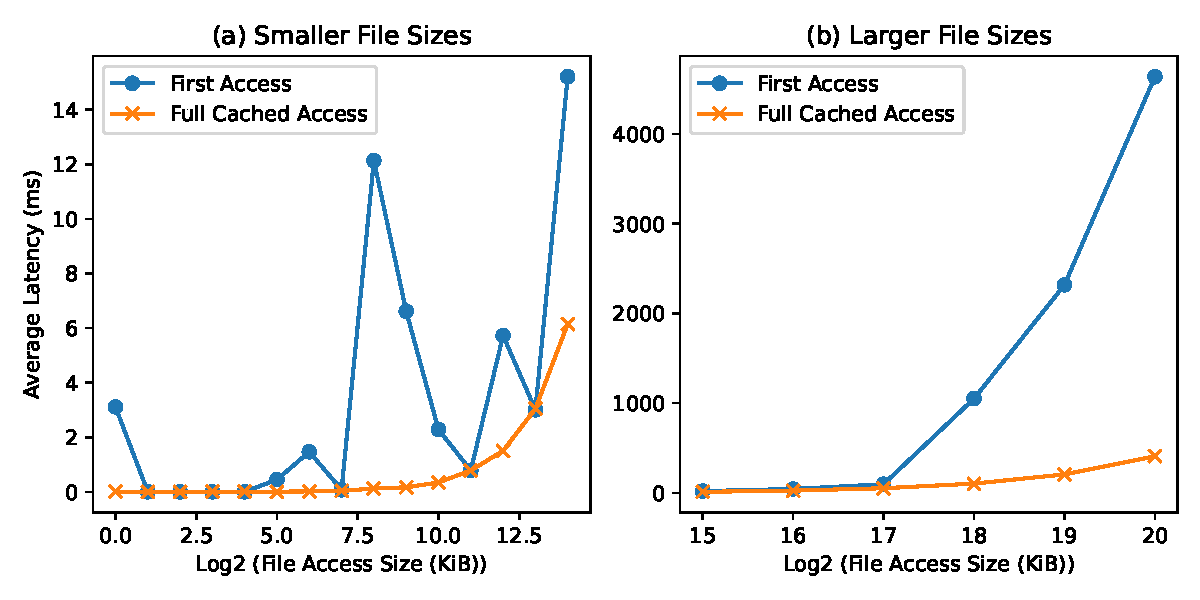
\includegraphics[width=0.98\linewidth]{sourcecode/file/filecache.pdf}
	\caption{\label{fig:file_cache} \textbf{File Cache Access}}
	%\vspace{-4mm}
\end{figure}
Figure~\ref{fig:file_cache} shows the results of file access time with increasing file access size. Since small file access and large file access show pretty different latencies. We split the results into two figures. Figure~\ref{fig:file_cache}(a) plots results under smaller file access sizes (from 1KiB to 8MiB) while Figure~\ref{fig:file_cache}(b) plots results under larger file access sizes (from 8MiB to 1GiB). By observing difference between first access (i.e., non-fully cached) and second access (i.e., full cached access), we can see the notable influence by OS file page cache. In full cached file access, the latencies are lower and more stable compared to first access (i.e., non-fully cached).

\paragraph{Results analysis.}
The analysis of the results underscores the significant role of the file system cache in optimizing read operations, especially as file sizes increase. For smaller files, the impact of caching is less pronounced, likely due to the lower overall read time. However, as file sizes grow, the benefits of caching become increasingly evident. The experiment highlights how the operating system dynamically allocates memory for caching, efficiently managing resources to balance performance with other system demands. This dynamic allocation is key in handling varying workloads, as seen in the significant improvement in read times for large, cached files. The results provide valuable insights into the behavior of file system caches and underscore their importance in system performance optimization, especially for applications dealing with large-scale file operations.

\subsection{File Read Time}
\paragraph{Methodology.}
The experimental methodology was designed to evaluate the average read times for 4 KB pages within an increasingly larger file access range, expanding from 4 KB to 1 GB. The aim was to reveal how the read times are affected as the file size grows, especially contrasting the behaviors of sequential and random access. In sequential reads, the access pattern remains linear irrespective of the file size, potentially benefiting from consistent data retrieval strategies. For random reads, the expansion in the file access range introduces more variability and randomness in access locations, expected to exhibit a more pronounced effect on read times due to increased randomness and seek times in larger files.

\paragraph{Experimental results.}
\begin{figure}[t]
	\centering
	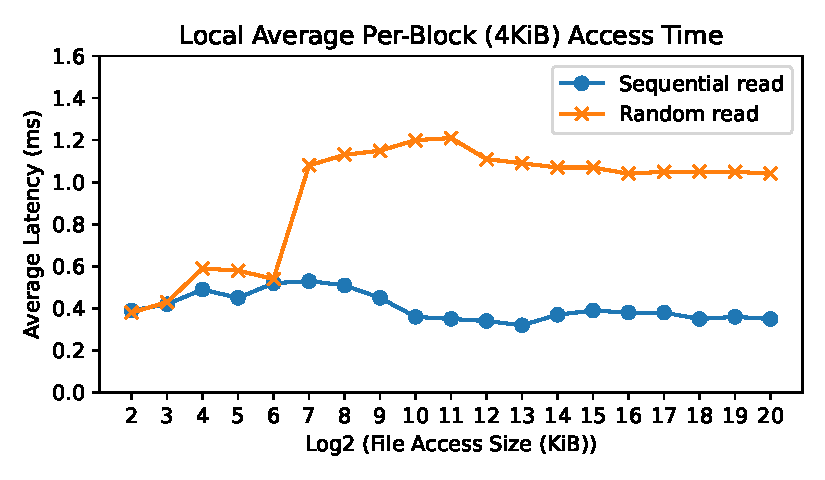
\includegraphics[width=0.98\linewidth]{sourcecode/file/file_direct.pdf}
	\caption{\label{fig:file_read_time} \textbf{File Read Time}}
	%\vspace{-4mm}
\end{figure}
Figure~\ref{fig:file_contention} plots the results of file read time with increasing file access region size.
The results show that with the increase in file size, the latency for sequential reads remain relatively stable with a slight decrease, suggesting a consistently efficient access pattern across various file sizes. In contrast, the read times for random access exhibits a notable increase as the file access range grew. This trend is more pronounced in larger file sizes, where the random nature of access leads to significantly higher read times compared to smaller sizes. The data highlight the impact of file size on read times, especially underlining the increasing inefficiency of random reads as the file size expanded.

\paragraph{Results analysis.}
These findings suggest that while sequential read operations maintain a relatively stable efficiency across different file sizes, random reads become increasingly inefficient with larger files. The stable performance of sequential reads can be attributed to the predictability and reduced seek times associated with linear data access. On the other hand, the increasing inefficiency observed in random reads for larger files is likely due to the higher seek times and the growing unpredictability in accessing data locations. This contrast in performance highlights the critical impact of file access patterns on read efficiency, particularly underlining the challenges in managing random reads in systems dealing with large files. This insight is essential for optimizing file system performance and can guide the design and optimization of data storage and retrieval strategies in large-scale data environments.

\subsection{Remote File Read Time}
\paragraph{Methodology.}
We use the same methodology and experimental program with local file read time experiment aforementioned. The only difference is that we use NFS instead of local filesystem on local disk. Therefore, we use another same virtual machine as NFS target and use our experimental to connect to NFS target. After that, we can see a NFS filesystem in our test machine. Finally, we run the same program to evaluate remote file read time on both random and sequential workloads.

\paragraph{Experimental results.}
\begin{figure}[t]
	\centering
	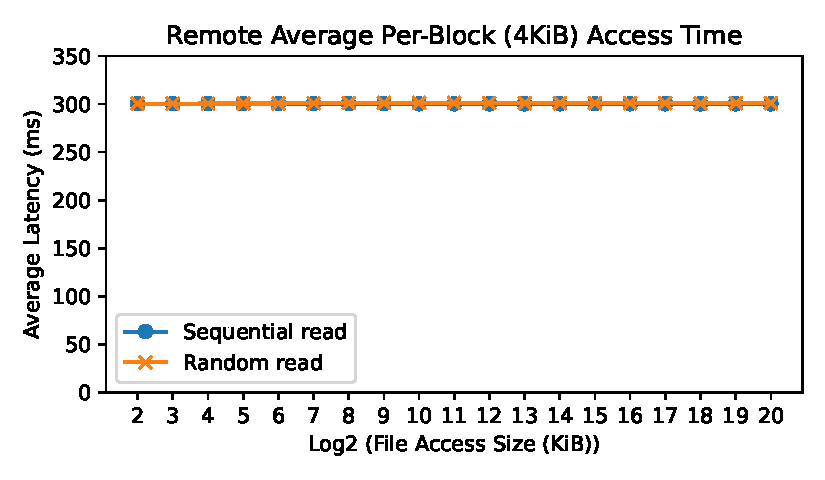
\includegraphics[width=0.98\linewidth]{sourcecode/file/file_remote.pdf}
	\caption{\label{fig:remote_file_read_time} \textbf{File Read Time}}
	%\vspace{-4mm}
\end{figure}
Figure~\ref{fig:remote_file_read_time} plots the results of remote file read time with increasing file access region size. The result is quite different with local file read time. In this remote access case, both random and sequential reads show almost same latency, which is pretty higher than local file read time. Even though we increase file access region size, the results do not show any difference.

\paragraph{Results analysis.}
From the results, we can get that reading remote file results in much higher latency than reading local file. This is because the network access time. The network access time is pretty higher than disk access time in our machines. Therefore, this leads to same access time for both sequential and random reads. This experiment tells us that in order to accelerate remote file access, both network and disk efficiency are equally important. We should optimize network and disk access efficiency together. 

\subsection{Contention}
\paragraph{Methodology.}
The experiment is designed to evaluate the concurrent read performance of a filesystem, particularly when multiple processes are simultaneously reading from different files on the same disk. The primary objective is to understand how increasing the number of processes affects the average read time for a single filesystem block. Our test program uses Direct I/O to bypass the file buffer cache, ensuring a more accurate measurement of disk access times. Each process reads 1024 blocks, each of 4096 bytes (typical filesystem block size), from a unique file. The read operations are performed randomly across the file to prevent sequential read optimizations and better mimic real-world access patterns. The experiment iterates over a varying number of processes, starting from 1 and going up to 16.
The total time taken for all reads in each process is then divided by the number of blocks to obtain the average block read time in milliseconds.

\paragraph{Experimental results.}
\begin{figure}[t]
	\centering
	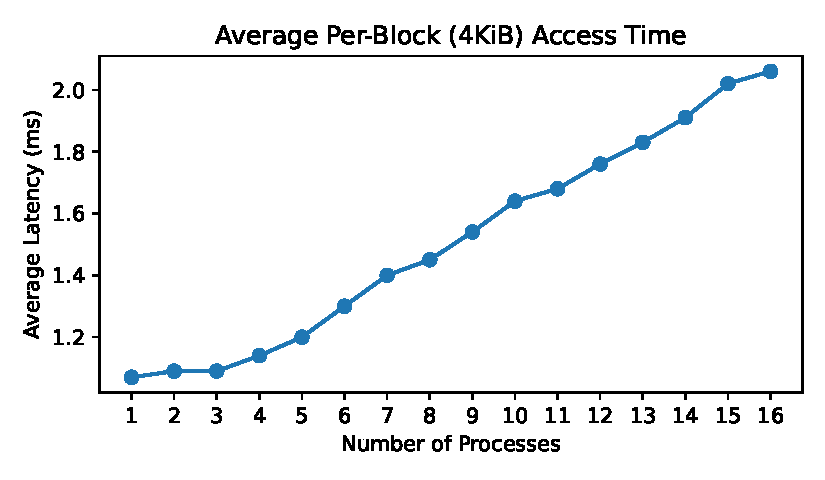
\includegraphics[width=0.98\linewidth]{sourcecode/file/file_contention.pdf}
	\caption{\label{fig:file_contention} \textbf{File Contention}}
	%\vspace{-4mm}
\end{figure}
Figure~\ref{fig:file_contention} plots the per-block (4KiB) access time under different concurrency. We can see that with the increasing of number of concurrent processes, the average per-block latency increases up to 2$\times$ (with 16 processes access simultaneously) compared to single process access.

\paragraph{Results analysis.}
The data indicates a clear trend: as the number of concurrent processes increases, the average time taken to read a single block also increases. This result is consistent with expectations, as more processes lead to increased contention for disk resources.

In the initial stages (1-4 processes), the increase in read time is relatively marginal, suggesting that the disk subsystem can handle low levels of concurrency without significant degradation in performance. However, beyond 4 processes, the read time starts increasing at a higher rate. This trend is more pronounced from 9 processes onwards, indicating a substantial contention in the disk subsystem.